\section{Página de previsualización de una ley de lex.gal}
\label{PPrevisualizacionLexGal}

\begin{figure}[H]
\centerline{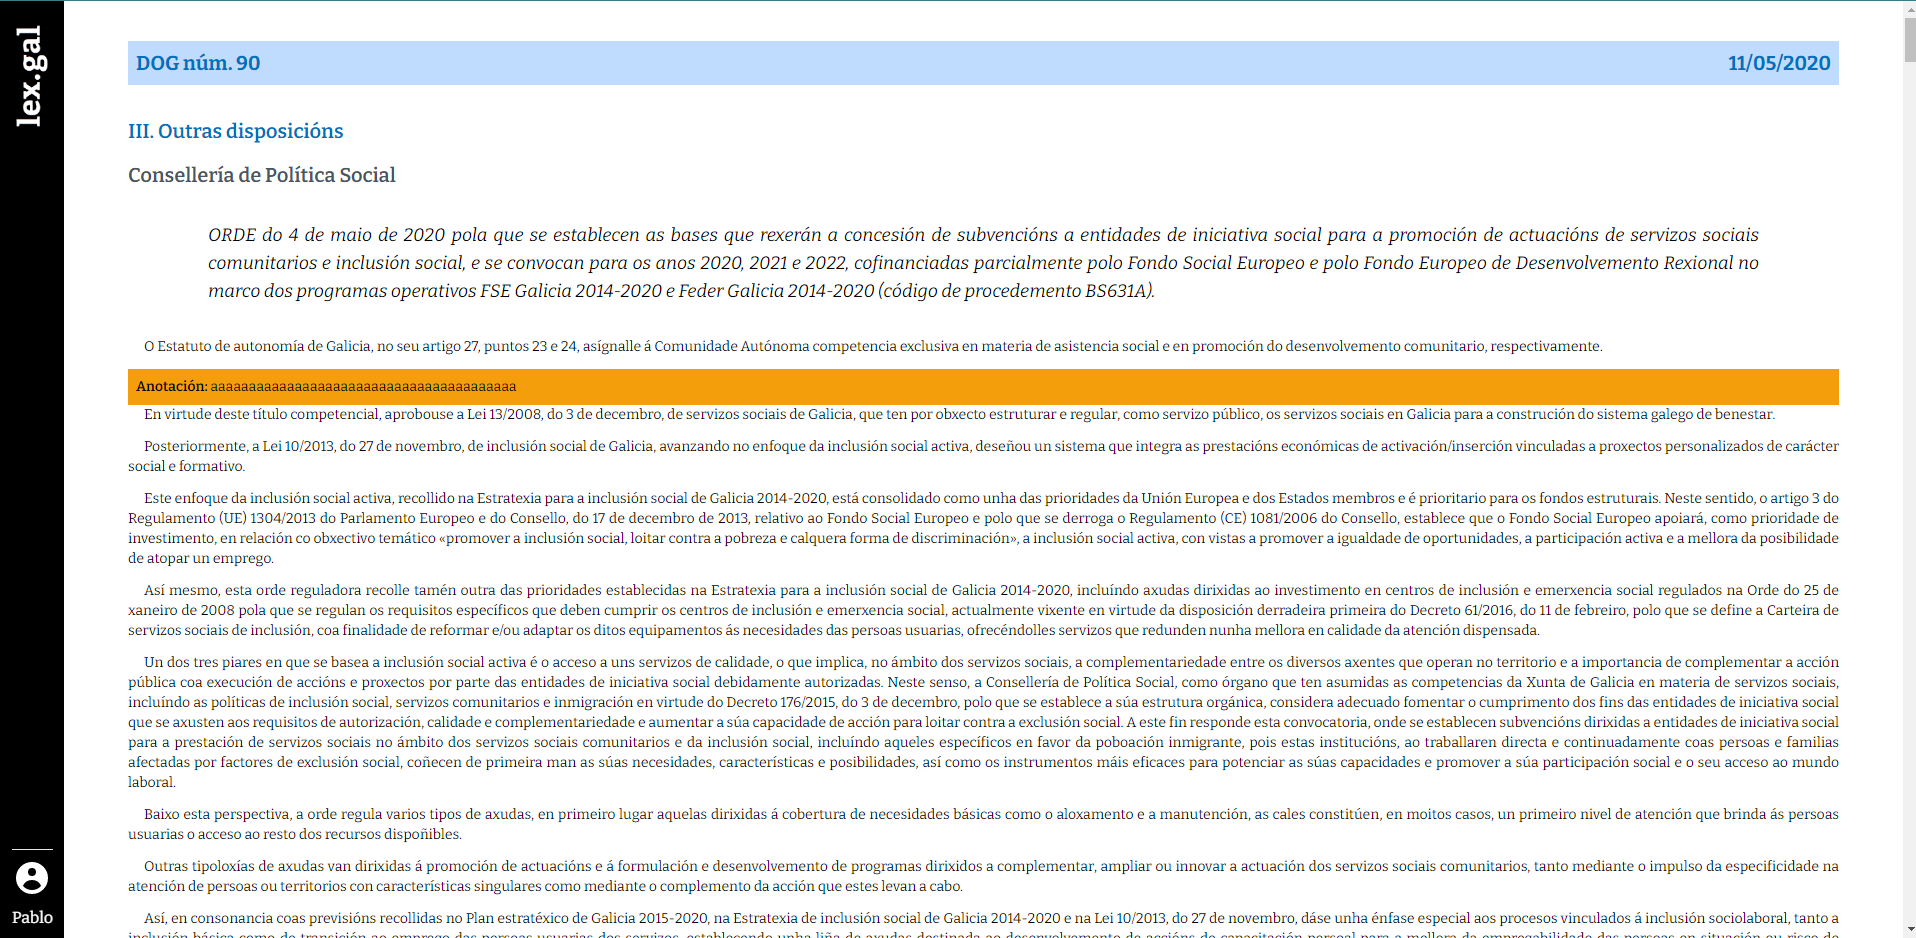
\includegraphics[width=15cm]{figuras/manualUsuario/PrevisualizarLEXGAL.PNG}}
\caption{Página de previsualización de una ley de lex.gal.}
\label{enlacePrevisualizacionLexGal}
\end{figure}

En esta página, mostrada en la \hyperref[enlacePrevisualizacionLexGal]{Figura B.8}, se puede previsualizar el contenido de una ley de lex.gal. Se mostrará en ella:
\begin{itemize}
    \item En el recuadro azul el número del DOG y la fecha de publicación en el DOG.
    \item Con color de letra azul el título de la sección a la que pertenece.
    \item Con color gris el publicador del documento.
    \item Con letra cursiva el título/sumario de la ley.
    \item En texto plano, el contenido de la propia ley.
    \item Con fondo naranja, las anotaciones realizadas sobre un párrafo de la ley.
\end{itemize}